\documentclass{article}
\usepackage{listings}
\usepackage{mathrsfs}
\usepackage[utf8]{inputenc}
\usepackage{amssymb}
\usepackage{lipsum}
\usepackage{amsmath}
\usepackage{fancyhdr}
\usepackage{geometry}
\usepackage{scrextend}
\usepackage[english,german]{babel}
\usepackage{titling}
\setlength{\droptitle}{-3cm}
\usepackage{tikz}
\usepackage{algorithm,algpseudocode}
\usepackage[doublespacing]{setspace}
\usetikzlibrary{datavisualization}
\usetikzlibrary{datavisualization.formats.functions}
\usepackage{polynom}
\usepackage{amsmath}
\usepackage{gauss}
\usepackage{tkz-euclide}
\usetikzlibrary{datavisualization}
\usetikzlibrary{datavisualization.formats.functions}
\author{
Alexander Mattick Kennung: qi69dube\\
Kapitel 1
}
\usepackage{import}
\date{\today}
\geometry{a4paper, margin=2cm}
\usepackage{stackengine}
\parskip 1em
\newcommand\stackequal[2]{%
  \mathrel{\stackunder[2pt]{\stackon[4pt]{=}{$\scriptscriptstyle#1$}}{%
  $\scriptscriptstyle#2$}}
 }
\makeatletter
\renewcommand*\env@matrix[1][*\c@MaxMatrixCols c]{%
  \hskip -\arraycolsep
  \let\@ifnextchar\new@ifnextchar
  \array{#1}}
\makeatother
\lstset{
  language=haskell,
}
\lstnewenvironment{code}{\lstset{language=Haskell,basicstyle=\small}}{}
\usepackage{enumitem}
\setlist{nosep}
\usepackage{titlesec}

\titlespacing*{\subsection}{0pt}{2pt}{3pt}
\titlespacing*{\section}{0pt}{0pt}{5pt}
\titlespacing*{\subsubsection}{0pt}{1pt}{2pt}
\title{Vorlesung 4}


\begin{document}
	\maketitle
	Ziel LGS $A\overline{x}=\overline{b}$\\
	$A\in\mathbb{R}^{n\times n}$ und $x,b\in\mathbb{R}^{n}$\\
	Inverse: $x = A^{-1}b$ ist aber langsam und numerisch hoch instabil\\
	Gauss Elim: standard für per-Hand lösen, geht auch am Computer, essentiell $LR$ Zerlegung.\\
	LR Zerlegung:\\
	$$A=\begin{bmatrix}1&4&2\\
		3&-2&2\\
		2&1&-1\end{bmatrix} \stackrel{II-3I, II-2I}{\to}
		\begin{bmatrix}1&4&2\\
		0&-14&-4\\
		0&-7&-5\end{bmatrix}\to
		\begin{bmatrix}1&4&2\\
		0&-14&-4\\
		0&0&-3\end{bmatrix}=R $$
		Dazu  $L_1=\begin{bmatrix}1&0&0\\
		-3&1&0\\
		-2&0&1\end{bmatrix}$ und $L_2 = \begin{bmatrix}1&0&0\\
		0&1&0\\
		0&-2&1\end{bmatrix}$
	Insgesamt wissen wir $R = L_2L_1A\to  (L_2L_1)^{-1} R = A\to L_1^{-1}L_2^{-1} R = A$\\
	Die absoluten Werte von L ändern sich beim invertiern nicht, aber die Werte unter der diagonale werden mal (-1) genommen.\\
	$L_1^{-1}=\begin{bmatrix}1&0&0\\
		3&1&0\\
		2&0&1\end{bmatrix}$\\
	und\\
	$L_2 = \begin{bmatrix}1&0&0\\
		0&1&0\\
		0&2&1\end{bmatrix}$
	Produkt aus beiden ist:\\
	$L=\begin{bmatrix}1&0&0\\
		3&1&0\\
		2&2&1\end{bmatrix}$\\
	Daraus folgt $A=LR$\\
	Zum lösen:\\
	$Ax = b \iff LRx = b$\\
	durch substitution $Rx = y$ entsteht $Ly = b$.\\
	$L\cdot y = b$\\
	Forwärtseinsetzen:\\
	$\begin{bmatrix}1&0&0\\
		3&1&0\\
		2&2&1\end{bmatrix}y = \begin{bmatrix}b_1\\b_2\\b_3\end{bmatrix}\implies y_1 = b_1, y_2=b_2-3y_1,\dots$\\
	und dann normal $Rx=y$ durch Rückwärtseinsetzen\\
	$\begin{bmatrix}1&4&2\\
		0&-14&-4\\
		0&0&-3\end{bmatrix}x = y$ und jetzt ganz normal.\\
	\section{Präsenzaufgabe 1}
	a) tridiagonale Matrix (kommt oft in z.B. diskretisierung von DGL vor)\\
	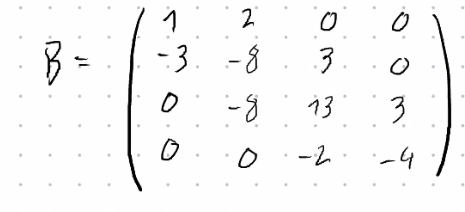
\includegraphics[width=256px]{tridiagonal.png}\\
	MAN ZIEHT IMMER ZEILEN AB. Der dafür benötigte Faktor kann dann direkt in die L matrix geschrieben werden, kein (-1)* notwendig.\\
	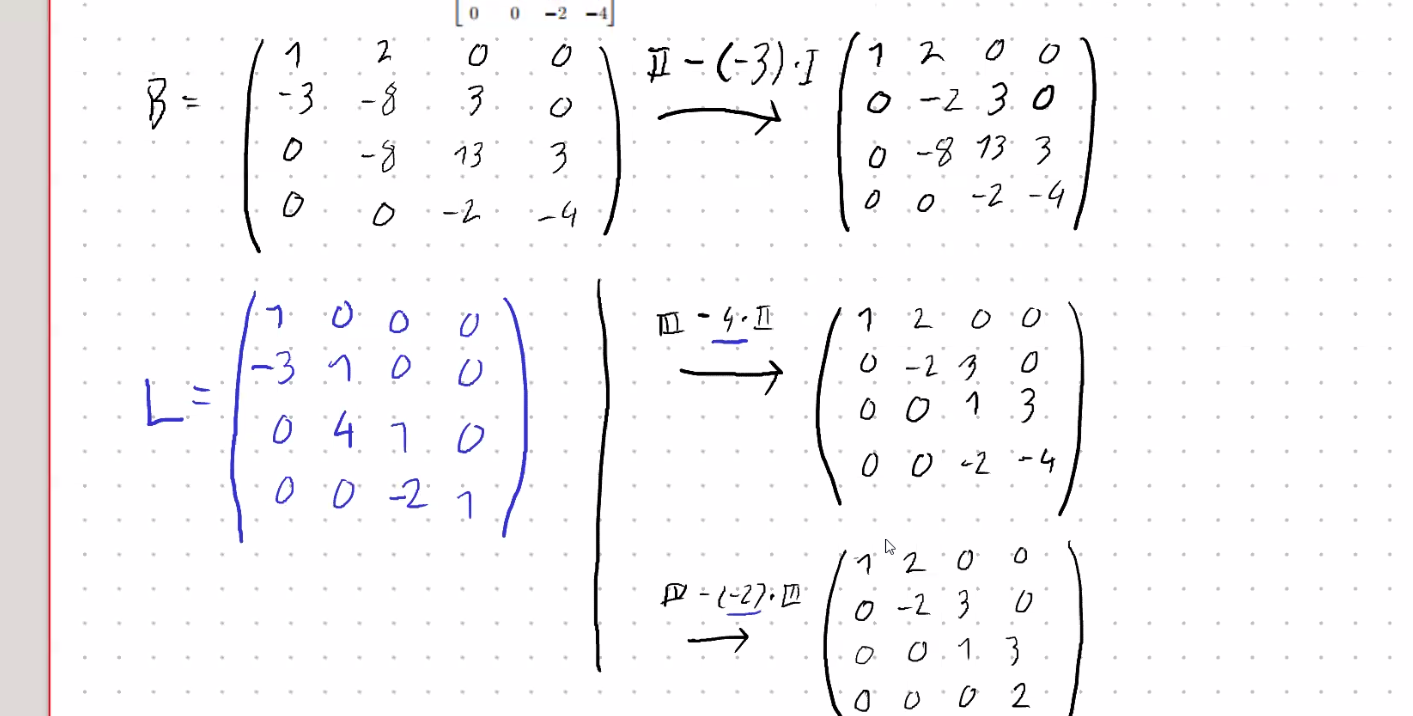
\includegraphics[width=256px]{LösungTridigonal.png}\\
	Struktur einer Tridiagonalen Matrixlösung:\\
	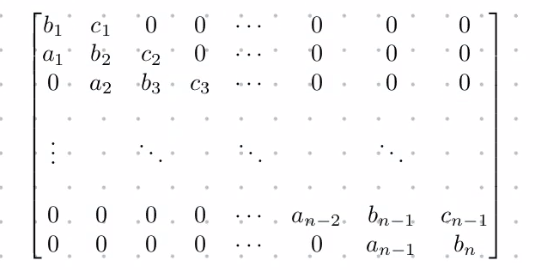
\includegraphics[width=256px]{tridigonalAbstract.png}\\
	$L =\begin{bmatrix}1&0&0&0&\hdots\\
		a_1&1&0&0&\hdots\\
		0&a_2&1&\dots&\hdots\\
		\hdots&\ddots&\ddots&\ddots&\hdots\end{bmatrix}$
	\\
	und
	$L =\begin{bmatrix}b_1&c_1&0&0&\hdots\\
		0&r_2&c_2&0&\hdots\\
		0&0&r_3&c_3&\hdots\\
		\hdots&\ddots&\ddots&\ddots&\hdots\end{bmatrix}$
	Wobei die c's einfach aus A übernommen werden können! (über ihnen sind ja immer nur nullen,also verändern sie sich nicht).\\
	Algorithmisch:\\
	Erste Zeile $r_1 = b_1$\\
	Zweite Zeile $a_1-l_1\cdot r_1 = 0\implies l_1 =\frac{a_1}{r_1}$ und $r_2 = b_2-l_1\cdot c_1$\\
	allgemeine Zeile:\\
	$r_1=b_1$\\
	Für $k=1,\dots,n-1$\\
	$l_k = a_k-\frac{a_k}{r_k}$\\
	$r_{k+1} = b_{k+1}-l_k\cdot c_k$\\
	Laufzeit: $O(n)$\\
	Aufwand des Lösens von $L\cdot y = b$, $R\cdot x = y$ bei tridiagonalen Matritzen\\
	Also:\\
	$y_1 = b_1$\\
	$y_2 = b_2-y_1\cdot l_1$\\
	Allgemein Algorithmus\\
	\begin{algorithmic}
	\State $y_1 = b_1$
	\For {$k=1,\dots, n-1$}
	\State $y_k =b_k-l_{k-1}y_{k-1}$
	\EndFor
	\end{algorithmic}
	$R\cdot x=y$\\
	$x_n = \frac{y_n}{r_n}$\\
	$x_{n-1} = \frac{y_{n-1}-c_{n-1}*x_{n}}{r_{n-1}}$
	Algorithmus:\\
	\begin{algorithmic}
	\State $x_n = \frac{y_n}{r_n}$
	\For {$k=n-1, \dots,1$}
	\State $x_k =\frac{y_{n-1}-c_{n-1}*x_{n}}{r_{n-1}}$
	\EndFor
	\end{algorithmic}
	QR Zerlegung: $Q$ Orthogonalmatrix.\\
	$R$ obere, rechte Dreiecksmatrix\\
	$QRx=b\iff Rx=Q^T b$\\
	Q Givensrotation und Housholder Spiegelungen.\\
	Ziel: Der i-te Eintrag der j-ten spalte von A zu null.\\
	$\to$ Nur die j-te spalte $A_j=\begin{bmatrix}a_{1,j}\\\hdots\\a_{j,j}\\\hdots\\a_{i,j}\\\hdots\end{bmatrix}$
	dafür einfach nur die digonale und und zu eliminierendes betrachten: $v=(a_{jj},a_{ij})^T$\\
	Zum lösen mit LR Zerlegung und pivot-matrix p $A=PLR$ muss man beim tauschen auch immer darauf achten, dass man die schon existierenden L-Spalten mittauscht:\\
	\begin{algorithm}
	\textbf{LR-Zerlegung mit Pivot}
	\begin{algorithmic}
	\Require $A\in\mathbb{R}^{n\times n}$
	\State $P\gets E_n$
	\State $L\gets\textbf{0}^{n\times n}$
	\For{$i\in[0..n]$}
		\State $pivot\gets$ pivot\_index(A,i)
		\State swap\_row(L,i,pivot)
		\State swap\_row(R,i,pivot)
		\State swap\_row(P,i,pivot)
		\State factor $\gets 1/A[i][i]$
		\For{$j\in[i..n]$}
			\State $l\gets A[i][j]*factor$
			\State $A[j]\gets A[j]-A[i]*l$
			\State $L[i][j]\gets l$
		\EndFor
	\EndFor\\
	\Return $P^T$, $E_n+L$, $A$ 
	\end{algorithmic}
	\end{algorithm}
\end{document}